\section{Petri nets}

\subsection{Overview}

\acrfull{PN} are a graphical and mathematical modeling tool
used to describe and analyze the behavior of concurrent systems.
They were introduced by the German researcher
Carl Adam Petri in his doctoral dissertation \cite{petri1962}
and have since been applied in a variety of fields
such as computer science, engineering, and biology.
A concise summary of the theory of Petri nets,
its properties, analysis, and applications can be found in \cite{murata1989}.

A Petri net is a bipartite, directed graph
consisting of a set of places, transitions, and arcs.
There are two types of nodes: places and transitions.
Places represent the state of the system,
while transitions represent events or actions that can occur.
Arcs connect places to transitions or transitions to places.
There can be no arcs between places nor transitions,
thus preserving the bipartite property.

Places may hold zero or more tokens.
Tokens are used to represent the presence or absence of entities in the system,
such as resources, data, or processes.
In the most simple class of Petri nets,
tokens do not carry any information and they are indistinguishable from one another.
The number of tokens at a place or the simple presence of a token is
what conveys meaning in the net.
Tokens are consumed and produced as transitions fire,
giving the impression that they move through the arcs.

In the conventional graphical representation,
places are depicted using circles, while transitions are depicted as rectangles.
Tokens are represented as black dots inside of the places,
as seen in Fig. \ref{fig:petri-net-example}.

\begin{figure}[!htb]
    \centering
    \includesvg[width=0.9\linewidth]{petri-net-example.svg}
    \caption{Example of a Petri net. \uppercase{PLACE 1} contains a token.}
    \label{fig:petri-net-example}
\end{figure}

When a transition fires, it consumes tokens from its input places and
produces tokens in its output places, reflecting a change in the state of the system.
The firing of a transition is enabled when there are sufficient tokens in its input places.
In Fig. \ref{fig:petri-net-transition-example}, we can see how successive firings happen.

\begin{figure}[!htb]
    \centering
    \includesvg[width=0.9\linewidth]{petri-net-transition-example.svg}
    \caption{Example of transition firing: Transition 1 fires first, then transition 2 fires.}
    \label{fig:petri-net-transition-example}
\end{figure}

The firing of enabled transitions is not deterministic,
i.e., they fire randomly as long as they are enabled.
A disabled transition is considered \emph{dead}
if there is no reachable state in the system that can lead to the transition being enabled.
If all the transitions in the net are dead, then the net is considered \emph{dead} too.
This state is analogous to the deadlock of a computer program.

Petri nets can be used to model and analyze a wide range of systems,
from simple systems with a few components to complex systems with many interacting components.
They can be used to detect potential problems in a system,
optimize system performance, and design and implement systems more effectively.

They can also be used to model industrial processes \cite{aalst1994putting},
to validate software requirements expressed as use cases \cite{silva2004applying}
or to specify and analyze real-time systems \cite{kavi1996specification}.

In particular, Petri nets can be used to detect deadlocks in source code
by modeling the input program as a Petri net and then analyzing the structure of the resulting net.
It will be shown that this approach is formally sound and
practicably amenable to source code written in the Rust programming language.

\subsection{Formal mathematical model}
\label{sec:petri-net-definition}

A Petri net is a particular kind of bipartite, weighted, directed graph,
equipped with an initial state called the \emph{initial marking}, $M_{0}$.
For this work, the following general definition of a Petri net
taken from \cite{murata1989} will be used.

\begin{definition}{Petri net}{petri-net}
    A Petri net is a 5-tuple, $ PN = (P, T, F, W, M_{0}) $ where:

    \begin{quote}
        $ P = \{ p_1, p_2, \dots, p_m \} $ is a finite set of places,\\
        $ T = \{ t_1, t_2, \dots, t_n \} $ is a finite set of transitions,\\
        $ F \subseteq (P \times T) \cup (T \times P) $ is a set of arcs (flow relation),\\
        $ W: F \leftarrow \{1, 2, 3, ... \} $ is a weight function for the arcs,\\
        $ M_{0}: P \leftarrow \{0, 1, 2, 3, .... \} $ is the initial marking,\\
        $ P \cap T = \varnothing $ and $ P \cup T \neq \varnothing $
    \end{quote}
\end{definition}

In the graphical representation, arcs are labeled with their weight,
which is a non-negative integer $k$.
Usually, the weight is omitted if it is equal to 1.
A $k$-weighted arc can be interpreted as a set of $k$ distinct parallel arcs.

A \emph{marking (state)} associates with each place a non-negative integer $l$.
If a marking assigns to place $p$ a non-negative integer $l$,
we say that $p$ is \emph{marked with $l$ tokens}.
Pictorially, we denote his by placing $l$ black dots (tokens) in place $p$.
The \emph{pth} component of $M$, denoted by $M(p)$, is the number of tokens in place $p$.

An alternative definition of Petri nets uses \emph{bags} instead of a set to define the arcs,
thus allowing multiple elements to be present.
It can be found in the literature, e.g., \cite[Definition 2.3]{peterson1981}.

As an example, consider the Petri net $ PN_{1} = (P, T, F, W, M) $ where:

\begin{quote}
    $ P = \{ p_1, p_2 \} $,\\
    $ T = \{ t_1, t_2 \} $,\\
    $ F = \{ (p_1, t_1), (p_2, t_2), (t_1, p_2), (t_2, p_2) \} $,\\
    $ W(a_i) = 1 \quad \forall a_i \in F $\\
    $ M(p_1) = 0, M(p_2) = 0 $
\end{quote}

This net contains no tokens and all the arc weights are equal to 1.
It is shown in Fig. \ref{fig:petri-net-formal-example}.

\begin{figure}[!htb]
    \centering
    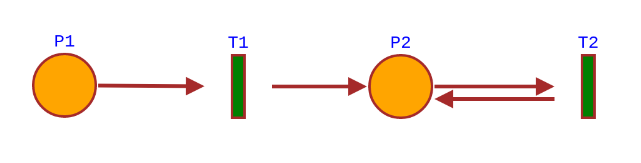
\includegraphics[scale=0.50]{petri-net-formal-example.png}
    \caption{Example of a small Petri net containing a self-loop.}
    \label{fig:petri-net-formal-example}
\end{figure}

Fig. \ref{fig:petri-net-formal-example} contains an interesting structure
that we will encounter later.
This motivates the following definition.

\begin{definition}{Self-loop}{self-loop}
    A place node $p$ and a transition node $t$ define a self-loop
    if $p$ is both an input place and an output place of $t$.
\end{definition}

In most cases, we are interested in Petri nets containing no self-loops,
which are called \emph{pure}.

\begin{definition}{Pure Petri net}{pure-petri-net}
    A Petri net is said to be pure if it has no self-loops.
\end{definition}

Moreover, if every arc weight is equal to one, we call the Petri net \emph{ordinary}.

\begin{definition}{Ordinary Petri net}{ordinary-petri-net}
    A Petri net is said to be ordinary if all of its arc weights are 1's, i.e.
    \begin{equation*}
        W(a) = 1 \quad \forall a \in F
    \end{equation*}
\end{definition}

\subsection{Transition firing}
\label{sec:transition-firing}

The transition firing rule is the core concept in Petri nets.
Despite being deceptively simple, its implications are far-reaching and complex.

\begin{definition}{Transition firing rule}{transition-firing-rule}
    Let $ PN = (P, T, F, W, M_{0}) $ be a Petri net.
    \begin{enumerate}[label=(\roman*)]
        \item A transition $t$ is said to be enabled if each input place $p$ of $t$
              is marked with at least $W(p, t)$ tokens,
              where $W(p,t)$ is the weight of the arc from $p$ to $t$.
        \item An enabled transition may or may not fire,
              depending on whether or not the event takes place.
        \item A firing of an enabled transition $t$ removes
              $W(t,p)$ tokens from each input place $p$ of $t$,
              where $W(t, p)$ is the weight of the arc from $t$ to $p$.
    \end{enumerate}
\end{definition}

Whenever several transitions are enabled for a given marking $M$,
any one of them can be fired.
The choice is nondeterministic.
Two enabled transitions are said to be in \emph{conflict}
if the firing of one of the transitions will disable the other transition.
In this case, the transitions compete for the token placed in a shared input place.

If two transitions $t_1$ and $t_2$ are enabled in some marking but are not in conflict,
they can fire in either order, i.e. $t_1$ then $t_2$ or $t_2$ then $t_1$.
Such transitions represent events that can occur concurrently or in parallel.
In this sense, the Petri net model adopts an \emph{interleaved model of parallelism}, that is,
the behavior of the system is the result of an arbitrary interleaving of the parallel events.

Transitions without input places or output places receive a special name.

\begin{definition}{Source transition}{source-transition}
    A transition without any input place is called a source transition.
\end{definition}

\begin{definition}{Sink transition}{sink-transition}
    A transition without any output place is called a sink transition.
\end{definition}

It is important to note that a source transition is unconditionally enabled
and produces tokens without consuming any, while the firing of a sink transition
consumes tokens without producing any.

\subsection{Online simulators}

To familiarize oneself with the dynamics of Petri nets,
it is useful to simulate some examples online
since seeing a Petri net in action is clearer than any static explanation on paper.
We have gathered some tools for this purpose to ease the burden on the reader.

\begin{itemize}
    \item A simple simulator by Igor Kim can be found on \url{https://petri.hp102.ru/}.
          A tutorial video on Youtube and example nets are included in the tool.
    \item A complement to this is a series of interactive tutorials by Prof. Wil van der Aalst
          at the University of Hamburg. These tutorials are Adobe Flash Player files (with extension \texttt{.swf})
          that modern web browsers cannot execute.
          Luckily, an online Flash emulator like the one found on \url{https://flashplayer.fullstacks.net/?kind=Flash_Emulator}
          can be used to upload the files and execute them.
    \item Another online Petri net editor and simulator is \url{http://www.biregal.com/}.
          The user can draw the net, add the tokens, and then manually fire transitions.
\end{itemize}

\subsection{Modeling examples}

In this subsection, several simple examples are presented to introduce
some basic concepts of Petri nets that are useful in modeling.
This subsection has been adapted from \cite{murata1989}.

For other modeling examples, such as the mutual exclusion problem,
semaphores as proposed by Edsger W. Dijkstra, the producer/consumer problem,
and the dining philosophers problem, the reader is referred to
\cite[Chap. 3]{peterson1981} and \cite{reisig2013}.

\subsubsection{Finite-state machines}

\acrfull{FSM} can be represented by a subclass of Petri nets.

As an example of a finite-state machine, consider a coffee vending machine.
It accepts \EUR{1} or \EUR{2} coins and sells two types of coffee,
the first costs \EUR{3} and the second \EUR{4}.
Assume that the machine can hold up to \EUR{4} and does not return any change.
Then, the state diagram of the machine can be represented
by the Petri net shown in Fig. \ref{fig:state-machine-example}.

\begin{figure}[!htb]
    \centering
    \includesvg[width=\linewidth]{state-machine-example.svg}
    \caption{The Petri net for a coffee vending machine.
        It is equivalent to a state diagram.}
    \label{fig:state-machine-example}
\end{figure}

The transitions represent the insertion of a coin of the labeled value,
e.g. ``Insert \EUR{1} coin''.
The places represent a possible state of the machine,
i.e. the amount of money currently stored inside.
The leftmost place labeled ``\EUR{0}'' is marked with a token
and corresponds to the initial state of the system.

We can now present the following definition of this subclass of Petri nets.

\begin{definition}{State machines}{state-machines}
    A Petri net in which each transition has exactly one incoming arc
    and exactly one outgoing arc is known as a state machine.

    Any \acrshort{FSM} (or its state diagram) can be modeled with a state machine.
\end{definition}

The structure of a place $p_1$ having two (or more) output transitions $t_1$ and $t_2$ is called
a \emph{conflict}, \emph{decision}, or \emph{choice}, depending on the application.
This is seen in the initial place of Fig. \ref{fig:state-machine-example},
where the user must select which coin to insert first.

\subsubsection{Parallel activities}

Contrary to finite-state machines, Petri nets can also model parallel or concurrent activities.
In Fig. \ref{fig:parallel-activities-example} an example of this is shown,
where the net represents the division of a bigger task
into two subtasks that may be executed in parallel.

\begin{figure}[!htb]
    \centering
    \includesvg[width=0.8\linewidth]{parallel-activities-example.svg}
    \caption{The Petri net depicting two parallel activities in a fork-join fashion.}
    \label{fig:parallel-activities-example}
\end{figure}

The transition ``Fork'' will fire before ``Task 1'' and ``Task 2''
and that ``Join'' will only fire after both tasks are complete.
But note that the order in which ``Tast 1'' and ``Tast 2'' execute is non-deterministic.
``Task 1'' could fire before, after, or at the same time that ``Task 2''.
It is precisely this property of the firing rule in Petri nets
that allows the modeling of concurrent systems.

\begin{definition}{Concurrency in Petri nets}{petri-net-concurrency}
    Two transitions are said to be concurrent if they are causally independent, i.e.
    the firing of one transition does not cause and is not triggered by the firing of the other.
\end{definition}

Note that each place in the net in Fig. \ref{fig:parallel-activities-example}
has exactly one incoming arc and one outgoing arc.
This subclass of Petri nets allows the representation of concurrency but not decisions (conflicts).

\begin{definition}{Marked graphs}{marked-graphs}
    A Petri net in which each place has exactly one incoming arc
    and exactly one outgoing arc is known as a marked graph.
\end{definition}

\subsubsection{Communication protocols}

Communications protocols can also be represented in Petri nets.
Fig. \ref{fig:communication-protocols-example} illustrates a simple protocol
in which Process 1 sends messages to Process 2 and
waits for an acknowledgment to be received before continuing.
Both processes communicate through a buffered channel whose maximum capacity is one message.
Therefore, only one message may be traveling between the processes at any given time.
For simplicity, no timeout mechanism was included.

\begin{figure}[!htbp]
    \centering
    \includesvg[width=\linewidth]{communication-protocols-example.svg}
    \caption{A simplified Petri net model of a communication protocol.}
    \label{fig:communication-protocols-example}
\end{figure}

A timeout for the send operation could be incorporated into the model
by adding a transition $t_{timeout}$ with edges from ``Wait for ACK'' to ``Ready to send''.
This maps the decision between receiving the acknowledgment and the timeout.

\subsubsection{Synchronization control}

In a multithreaded system, resources and information are shared among several threads.
This sharing must be controlled or synchronized
to ensure the correct operation of the overall system.
Petri nets have been used to model a variety of synchronization mechanisms,
including the mutual exclusion, readers-writers, and producers-consumers problems \cite{murata1989}.

A Petri net for a readers-writers system with $k$ processes
is shown in Fig. \ref{fig:readers-writers-example}.
Each token represents a process and the choice of T1 or T2
represents whether the process performs a read or a write operation.

It makes use of weighted edges to remove atomically
$k - 1$ tokens from P3 before performing a write (transition T2),
thus ensuring that no readers are present in the right loop of the net.

At most $k$ processes may be reading at the same same,
but when one process is reading, no process is allowed to read, that is P2 will be empty.
It can be easily verified that the mutual exclusion property is satisfied for the system.

\begin{figure}[!htbp]
    \centering
    \includesvg[width=\linewidth]{readers-writers-example.svg}
    \caption{A Petri net system with k processes that either read or write.}
    \label{fig:readers-writers-example}
\end{figure}

It should be pointed out that this system is not free from starvation,
since there is no guarantee that a write operation will eventually take place.
The system is on the other hand free from deadlocks.

\subsection{Important properties}

In this subsection, we will look at important concepts for the analysis of Petri nets
that will facilitate the understanding of the nets we will be dealing with in the rest of the work.

\subsubsection{Reachability}
\label{sec:reachability}

Reachability is one of the most important questions
when studying the dynamic properties of a system.
The firing of enabled transitions causes changes in the location of the tokens.
In other words, it changes the marking $M$.
A sequence of firings creates a sequence of markings
where each marking may be denoted as a vector of length $n$,
with $n$ being the number of places in the Petri net.

A \emph{firing} or \emph{occurence sequence} is denoted by
$ \sigma = M_0\; t_1\; M_1\; t_2\; M_2\; \cdots\; t_l\; M_l$ or simply
$ \sigma = t_1\; t_2\; \cdots\; t_l\; $, since the markings
resulting from each firing are derived
from the transition firing rule described in Sec. \ref{sec:transition-firing}.

\begin{definition}{Reachability}{reachability}
    We say that a marking $M$ is reachable from $M_0$
    if there exists a firing sequence $\sigma$ such that $M$ is contained in $\sigma$.
\end{definition}

The set of all possible markings reachable from $M_0$ is denoted by $R(N, M_0)$ or more simply
$R(M_0)$ when the net meant is clear.
This set is called the \emph{reachability set}.

A problem of utmost importance in the theory of Petri nets can be presented then,
namely the \emph{reachability problem}:
Finding if $M_n \in R(M_0, N)$ for a given net and initial marking.

In some applications, we are just interested in the markings of a subset of places
and we can ignore the remaining ones.
This leads to a variation of the problem known as the \emph{submarking reachability problem}.

It has been shown that the reachability problem is decidable \cite{mayr1981}.
Nevertheless, it was also shown that it takes exponential space
(formally, it is EXPSPACE-hard) \cite{lipton1976}.
New methods have been proposed to make the algorithms more efficient \cite{kungas2005petri}.
Recently, \cite{czerwinski2020reachability} improved
the lower bound and showed that the problem is not ELEMENTARY.
These results highlight that the reachability problem is still
an active area of research in theoretical computer science.

For this and other key problems, the most important theoretical results
obtained up to 1998 are detailed in \cite{esparza1994decidability}.

\subsubsection{Boundedness and safeness}

During the execution of a Petri net, tokens may accumulate in some places.
Applications need to ensure that the number of tokens in a given place does not
exceed a certain tolerance.
For example, if a place represents a buffer,
we are interested that the buffer will never overflow.

\begin{definition}{Boundedness}{boundedness}
    A place in a Petri net is k-bounded or k-safe
    if the number of tokens in that place cannot exceed a finite integer $k$
    for any marking reachable from $M_0$.

    A Petri net is k-bounded or simply bounded if all places are bounded.
\end{definition}

Safeness is a special case of boundedness.
It occurs when the place contains either 1 or 0 tokens during execution.

\begin{definition}{Safeness}{safeness}
    A place in a Petri net is safe if the number of tokens in that place never exceeds one.

    A Petri net is safe if each place in that net is safe.
\end{definition}

The nets in Fig. \ref{fig:state-machine-example}, \ref{fig:parallel-activities-example}
and \ref{fig:communication-protocols-example} are all safe.

The net in Fig. \ref{fig:readers-writers-example}
is k-bounded because all its places are k-bounded.

\subsubsection{Liveness}

The concept of liveness is analogous to
the complete absence of deadlocks in computer programs.

\begin{definition}{Liveness}{liveness}
    A Patri net $(N, M_0)$ is said to be live
    (or equivalently $M_0$ is said to be a live marking for N) if,
    for every marking reachable from $M_0$, it is possible to fire any transition
    of the net by progressing through some firing sequence.
\end{definition}

When a net is live, it can always continue executing,
no matter the transitions that fired before.
Eventually, every transition can be fired again.
If a transition can be fired only once and there is no way to enable it again,
then the net is not live.

This is equivalent to saying that the Petri net is \emph{deadlock-free}.
Let us now define what constitutes a deadlock and show examples of it.

\begin{definition}{Deadlock in Petri nets}{petri-net-deadlock}
    A deadlock in a Patri net is a transition (or a set of transitions) that cannot fire
    for any marking reachable from $M_0$.
    The transition (or a set of transitions) cannot become enabled again
    after a certain point in the execution.
\end{definition}

A transition is \emph{live} if it is not deadlocked.
If a transition is live, it is always possible to pick a suitable firing
to get from the current marking to a marking that enables the transition.

The nets in Fig. \ref{fig:state-machine-example}, \ref{fig:parallel-activities-example}
and \ref{fig:communication-protocols-example} are all live.
In all these cases, after some firings,
the net returns to the initial state and can restart the cycle.

The net in Fig. \ref{fig:petri-net-example} is not live.
After two firings it finishes executing and nothing more can happen.
The net in Fig. \ref{fig:petri-net-formal-example} is also not live, because
T1 will only execute once and only T2 can be enabled from that point on.

\subsection{Reachability Analysis}

Having introduced the reachability set $R(N, M_0)$ in Sec. \ref{sec:reachability},
we can now present a major analysis technique for Petri nets: the \emph{reachability tree}.

We will run the algorithm for constructing the reachability tree step by step
and then present its advantages and drawbacks.
In general terms, the reachability tree has the following structure:
Nodes represent markings generated from $M_0$, the root of the tree, and its successors.
Each arc represents a transition firing, which transforms one marking into another.

\begin{figure}[!htb]
    \centering
    \includesvg[width=0.5\linewidth]{reachability-tree-example.svg}
    \caption{A marked Petri net for illustrating the construction of a reachability tree.}
    \label{fig:reachability-tree-example}
\end{figure}

Consider the Petri net shown in Fig. \ref{fig:reachability-tree-example}.
The initial marking is $(1, 0, 0)$.
In this initial marking, two transitions are enabled: T1 and T3.
Given that we would like to obtain the entire reachability set,
we define a new node in the reachability tree for each reachable marking,
which results from firing each transition.
An arc, labeled by the transition fired, leads from the initial marking
(the root of the tree) to each of the new markings.
After this first step (Fig. \ref{fig:reachability-tree-step-1}),
the tree contains all markings that are immediately reachable from the initial marking.

\begin{figure}[!htb]
    \centering
    \includesvg[width=0.5\linewidth]{reachability-tree-step-1.svg}
    \caption{The first step building the reachability tree
        for the Petri net in Fig. \ref{fig:reachability-tree-example}.}
    \label{fig:reachability-tree-step-1}
\end{figure}

Now we must consider all markings reachable from the leaves of the tree.

From marking $(0,0,1)$ we cannot fire any transition.
This is known as a \emph{dead marking}.
In other words, it is a ``dead-end'' node.
This class of end-states is particularly relevant for deadlock analysis.

From the marking on the right of the tree, denoted $(1, 1, 0)$, we can fire T1 or T3.
If we fire T1, we obtain $(0, 1, 1)$ and if T3 fires, the resulting marking is $(1, 2, 0)$.
This produces the tree of Fig. \ref{fig:reachability-tree-step-2}.

\begin{figure}[!htb]
    \centering
    \includesvg[width=0.7\linewidth]{reachability-tree-step-2.svg}
    \caption{The second step building the reachability tree
        for the Petri net in Fig. \ref{fig:reachability-tree-example}.}
    \label{fig:reachability-tree-step-2}
\end{figure}

Note that starting with marking $(0, 1, 1)$, only the transition T2 is enabled,
which will lead to a marking $(0, 0, 1)$ that was already seen before.
If instead we take $(1, 2, 0)$ we have again the same possibilities as starting from $(1, 1, 0)$.
It is easy to see that the tree will continue to grow down that path.
The tree is therefore infinite and this is because
the net in Fig. \ref{fig:reachability-tree-example} is not bounded.
See Fig. \ref{fig:reachability-tree-final-step} for the abbreviated final result.

\begin{figure}[!htb]
    \centering
    \includesvg[width=\linewidth]{reachability-tree-final-step.svg}
    \caption{The infinite reachability tree for the Petri net in Fig.
        \ref{fig:reachability-tree-example}.}
    \label{fig:reachability-tree-final-step}
\end{figure}

The previously presented method enumerates the elements in the reachability set.
Every marking in the reachability set will be produced
and so for any Petri net with an infinite reachability set
(i.e. an infinite number of possible states),
the corresponding tree would also be infinite.
Nonetheless, this opposite is not true.
A Petri net with a finite reachability set can have an infinite tree
(see Fig. \ref{fig:reachability-tree-bounded-net-counterexample}).
This net is even \emph{safe}.
In conclusion, dealing with a bounded or safe net is not
a guarantee that the total number of reachable states will be finite.

\begin{figure}[!htb]
    \centering
    \includesvg[width=0.9\linewidth]{reachability-tree-bounded-net-counterexample.svg}
    \caption{A simple Petri net with an infinite reachability tree.}
    \label{fig:reachability-tree-bounded-net-counterexample}
\end{figure}

For the reachability tree to be a useful analysis tool,
it is necessary to devise a method to limit it to a finite size.
This implies in general a certain loss of information since the method will have to map
an infinite number of reachable markings onto a single element.
The reduction to a finite representation may be accomplished by the following means.

Notice on one hand that we may encounter duplicate nodes
in our tree and we always naively treat them as new.
This is illustrated most clearly in Fig. \ref{fig:reachability-tree-bounded-net-counterexample}.
It is thus possible to stop the exploration of the successors of a duplicated node.

Notice on the other hand that some markings are strictly different from previously seen markings
but they enable the same set of transitions.
We say in this case that the marking with additional tokens \emph{covers} the one
that has the minimum number of tokens needed to enable the set of transitions in question.
Firing some transitions may allow us to accumulate an arbitrary number of tokens in one place.
For example, firing T3 in the Petri net seen in
Fig. \ref{fig:reachability-tree-example} exhibits exactly this behavior.
Therefore, it would suffice to mark the accumulating place
with a special label $\omega$, which stands for infinity
since we could get as many tokens as we wish in that place.

For instance, the result of converting the tree of Fig. \ref{fig:reachability-tree-final-step}
to a finite tree is shown in Fig. \ref{fig:reachability-tree-final-step-finite}.

\begin{figure}[!htb]
    \centering
    \includesvg[width=0.7\linewidth]{reachability-tree-final-step-finite.svg}
    \caption{The finite reachability tree for the Petri net in Fig.
        \ref{fig:reachability-tree-example}.}
    \label{fig:reachability-tree-final-step-finite}
\end{figure}

For more details about

\begin{enumerate}
    \item the technique for representing infinite reachability trees using $\omega$,
    \item a definition of the algorithm and precise steps for constructing the reachability tree,
    \item mathematical proof that the reachability tree generated by it is finite,
    \item and the distinction between the reachability tree and the \emph{reachability graph}
\end{enumerate}

the reader is referred to \cite{murata1989} and \cite{peterson1981}.
These concepts are beyond the scope of this work
and are not required in the following chapters.